%% ICAIF '26 poster for "Making Tail Constraints Bind" (paper 873).
%% A0 portrait (84.1 x 118.9 cm), as required by the organisers.
%% Style follows the Columbia MAFN posters: full-width blue title banner with
%% logos, two plain columns, centred bold section headings. Text and math are set in
%% STIX Two, the same family as the figures.
%% Build: cd poster && latexmk -pdf poster.tex
%% Figures: poster versions of the paper's figures from scripts/make_poster_figures.py, in the
%% style of scripts/_poster_style.py (poster/figures/, found before ../paper/figures/ on the
%% graphics path). Logos live in logos/.
%% Every number on the poster is taken from paper/main.tex or that script.
\documentclass[25pt, a0paper, portrait, margin=0mm, innermargin=25mm,
  blockverticalspace=6mm, colspace=25mm, subcolspace=8mm]{tikzposter}

\usepackage[T1]{fontenc}
\usepackage{amsmath}
\usepackage{amssymb}
\usepackage{stix2}
\usepackage{booktabs}
\usepackage{array}
\usepackage{graphicx}
\usepackage{enumitem}
\usepackage{ragged2e}
\usetikzlibrary{arrows.meta, positioning, calc}
\graphicspath{{figures/}{../paper/figures/}{logos/}}

%% ---------------------------------------------------------------------------
%% Palette. The banner is the slate navy of the 2025 MAFN cohort posters; the MAFN crown tile
%% is recoloured to match (logos/mafn_navy.png). Headings and highlights use a deeper blue
%% than the figures' accent so that text keeps its contrast.
\definecolor{ink}{HTML}{222222}
\definecolor{navy}{HTML}{0F4D92}
\definecolor{banner}{HTML}{2F4B7C}
\definecolor{dark}{HTML}{4D4D4D}
\definecolor{mid}{HTML}{8C8C8C}
\colorlet{tint}{navy!7}

\usetheme{Default}
\usetitlestyle{Filled}
\colorlet{backgroundcolor}{white}
\colorlet{framecolor}{white}
\colorlet{titlefgcolor}{white}
\colorlet{titlebgcolor}{banner}
\colorlet{blocktitlebgcolor}{white}
\colorlet{blocktitlefgcolor}{navy}
\colorlet{blockbodybgcolor}{white}
\colorlet{blockbodyfgcolor}{ink}

%% Sections: centred bold heading over a thin navy rule, no frame or fill.
\defineblockstyle{Plain}{
  titlewidthscale=1, bodywidthscale=1, titlecenter,
  titleoffsetx=0pt, titleoffsety=0pt, bodyoffsetx=0pt, bodyoffsety=0pt,
  bodyverticalshift=0pt, roundedcorners=0, linewidth=0pt,
  titleinnersep=3.5mm, bodyinnersep=2mm
}{
  \ifBlockHasTitle
    \draw[navy, line width=0.5mm] (blocktitle.south west) -- (blocktitle.south east);
  \fi
}
\useblockstyle{Plain}
\tikzposterlatexaffectionproofoff

%% ---------------------------------------------------------------------------
\newcommand{\hl}[1]{\textcolor{navy}{\textbf{#1}}}
\newcommand{\runin}[1]{\par\smallskip\noindent\textcolor{navy}{\textbf{#1.}}\ }
\newcommand{\keynote}[1]{\par\smallskip\noindent{\setlength{\fboxsep}{4mm}\colorbox{tint}{%
  \begin{minipage}{\dimexpr\linewidth-8mm}\RaggedRight\itshape #1\end{minipage}}}\par}
\newcommand{\fig}[2][0.78\linewidth]{\par\smallskip{\centering
  \includegraphics[width=#1]{#2}\par}}
%% Key results under the abstract: a large navy number over a one-line label, thin rules between.
\newcommand{\keystat}[2]{\begin{minipage}[t]{0.31\linewidth}\centering
  {\fontsize{50}{58}\selectfont\bfseries\color{navy}#1\par}\vspace{2mm}
  {\fontsize{19}{23}\selectfont\color{dark}#2\par}\end{minipage}}
\newcommand{\keyrule}{\hfill{\color{navy!35}\rule[-24mm]{0.5mm}{36mm}}\hfill}
%% Envelope drawn in TikZ, so the poster needs no icon font.
\newcommand{\envelope}{\tikz[baseline=-0.1ex, line width=0.25mm, line join=round]{%
  \draw (0,0) rectangle (0.95em,0.62em); \draw (0,0.62em) -- (0.475em,0.25em) -- (0.95em,0.62em);}}
\newcommand{\figcap}[1]{{\centering\fontsize{19}{23}\selectfont\color{dark}#1\par}\smallskip}
\newcommand{\tabcap}[1]{{\centering\fontsize{19}{23}\selectfont\color{dark}#1\par}\smallskip}
\setlist{leftmargin=1.3em, itemsep=1mm, topsep=1mm, before=\RaggedRight}
%% Block bodies default to \large; academic density wants smaller type.
\newcommand{\body}{\fontsize{21}{26}\selectfont\setlength{\parskip}{0.4em}}
\renewcommand{\arraystretch}{1.05}


%% ---------------------------------------------------------------------------
\newlength{\logoh}\setlength{\logoh}{62mm}
\settitle{%
  \begin{minipage}[c]{0.17\linewidth}\centering
    
\includegraphics[height=\logoh]{logos/mafn_navy.png}
  \end{minipage}\hfill
  \begin{minipage}[c]{0.64\linewidth}\centering\color{white}
    {\fontsize{60}{72}\selectfont\bfseries Making Tail Constraints Bind: Two Silent Failure
      Modes in CVaR-Constrained Portfolio RL\par}
    \vspace{9mm}
    {\LARGE Nigel Li\qquad Yutong Han\par}
    \vspace{4mm}
    {\large\itshape Columbia University, New York\par}
  \end{minipage}\hfill
  \begin{minipage}[c]{0.17\linewidth}\centering
    
\includegraphics[height=\logoh]{logos/icaif_white.png}
  \end{minipage}}

\begin{document}
\maketitle[innersep=9mm, titletoblockverticalspace=6mm]

\begin{columns}
%% ===========================================================================
\column{0.5}
\block{Abstract}{\body
  Reinforcement learning (RL) portfolio allocators are often given a tail-risk limit through a
  Lagrangian penalty on Conditional Value-at-Risk (CVaR). We show two ways in which this limit
  fails with no visible symptom, and fix them by scaling the dual step to the CVaR excess and
  adding a decision-time filter that moves each over-budget portfolio toward minimum variance
  before it trades.
  \par\medskip
  {\centering
  \keystat{7.4\%}{out-of-sample breach rate with\\ the filter, down from 75.1\%}\keyrule
  \keystat{26 of 27}{untied walk-forward folds with lower\\ $\mathrm{CVaR}_{0.99}$, $p=8.8\times10^{-6}$}\keyrule
  \keystat{7.7\%}{drawdown in March 2020, against\\ 16.3\% without the constraint}\par}
}

\block{Motivation}{\body
  In mid-March 2020 the S\&P 500 lost about 15\% in a single week. An RL allocator trained
  only to maximise return stayed in equities and fell 16.3\% from its peak. The same allocator
  with a limit on its tail losses had already moved into Treasuries and cash and fell 7.7\%
  (Fig.~1). One crash is a single case, so Figure 8 repeats the comparison over calm,
  high-volatility and selloff weeks, where the limit also cut tail losses.
  \fig[0.78\linewidth]{figure_stress_paths.pdf}
  \figcap{Figure 1. Drawdown over 2020 to 2024. Thick lines are five-seed means and thin lines
  individual seeds. Shaded, the drawdown the constraint avoided.}
}

\block{Problem and measures}{\body
  $\mathrm{CVaR}_\alpha$ is the average loss in the worst $(1-\alpha)$ share of weeks [1]. With
  $\alpha=0.95$ it averages the worst 5\%, so it measures how large the losses are beyond the
  Value-at-Risk (VaR) threshold (Fig.~2).
  \fig[0.78\linewidth]{figure_cvar_tail.pdf}
  \figcap{Figure 2. Weekly returns on the stress window, five seeds pooled. Shaded, the worst
  5\% of constrained weeks. Lines sit at minus each CVaR.}
  Each week the allocator chooses long-only weights $w_t$ on seven ETFs (SPY, TLT, HYG, DBC,
  GLD, UUP, BIL), using 887 weekly returns from 2008 to 2024. The problem is a constrained
  Markov decision process [2],
  \[
    \max_\pi\ J(\pi)\quad\text{s.t.}\quad \mathrm{CVaR}_{0.95}(L)\le d=1.2\%,\qquad
    \mathrm{CVaR}_\alpha(L)=\min_{\zeta\in\mathbb{R}}\Big\{\zeta+\tfrac{1}{1-\alpha}\,
      \mathbb{E}\big[(L-\zeta)^{+}\big]\Big\}.
  \]
  A test week is a breach when the trailing 52-week $\mathrm{CVaR}_{0.95}$ exceeds $d$, so the
  breach rate over the test weeks $\mathcal{T}$ is
  \[
    B=\frac{1}{|\mathcal{T}|}\sum_{t\in\mathcal{T}}
      \mathbf{1}\big[\widehat{\mathrm{CVaR}}_{0.95}(r_{t-52:t-1})>d\big],
  \]
  with 5\% of weeks tolerated. Sharpe ratios are annualised from weekly net returns, and their
  significance is judged with the Probabilistic and Deflated Sharpe ratios [4].
}

\block{Failure 1. The penalty weight never moves}{\body
  With a dual step $\eta_\lambda=10^{-3}$, $\lambda$ stayed near zero for all 1500 training
  updates (Fig.~3). The CVaR excess is about $10^{-2}$ per week, so each update moved
  $\lambda$ by about $10^{-5}$. Starting from $\lambda_0=0$, after $K$ updates
  \[
    \lambda_K\;\le\;\eta_\lambda\sum_{k=1}^{K}\big(\widehat{\mathrm{CVaR}}_k-d\big)^{+}
    \;\approx\;10^{-3}\cdot1500\cdot10^{-2}\;\approx\;10^{-2},
  \]
  and the trained value was 0.022. With $\eta_\lambda=5.0$, $\lambda$ rose to between 0.1 and
  0.3. A model-free actor-critic failed in the same way when its cost signal (about
  $10^{-3}$) was left unstandardised next to a unit-scale reward signal.
  \fig[0.78\linewidth]{figure_lambda_trace.pdf}
  \figcap{Figure 3. The penalty weight $\lambda$ during training, five seeds.}
  Tail metrics do not reveal the failure. Even with $\lambda$ near zero, the rest of the
  pipeline (the anchor, the projection and checkpoint selection under the CVaR limit) lowered
  $\mathrm{CVaR}_{0.99}$ by 61\% against the unconstrained learner (0.025 against 0.065,
  permutation test $p=0.0044$).
  \runin{Remedy} The multiplier should be monitored during training, since a value that remains
  at zero indicates an inactive constraint, and the dual step should be set on the scale of the
  CVaR excess. With $\eta_\lambda=5.0$ the penalty binds in training, although the portfolio
  still exceeds its budget out of sample. The decision-time filter addresses this residual
  breach.
}

\block{Failure 2. The test protocol reverses the ranking}{\body
  A walk-forward test retrains the model on a rolling window and evaluates it on the next
  unseen block. On a 31-asset universe, one fixed stress split ranked the constrained learner
  above minimum variance (Sharpe 0.85 against 0.23). A 20-fold walk-forward reversed the order
  (0.74 against 1.40, Fig.~4). With Ledoit-Wolf shrinkage [5], minimum variance still reached
  only 0.25 on the split. The tail-risk reduction against unconstrained RL held under both
  tests (fold-level Wilcoxon $p=6\times10^{-4}$).
  \fig[0.72\linewidth]{figure_protocol.pdf}
  \figcap{Figure 4. The same four methods ranked by two tests, 31-asset universe.}
  \runin{Remedy} Learned allocators should be compared with classical optimisers on rolling
  walk-forward folds, with multiple-testing control and the Deflated Sharpe ratio [4]. The
  Results section reports both protocols.
}

%% ===========================================================================
\column{0.5}
\block{Our method}{\body
  We train the allocator end to end with a CVaR penalty whose dual step matches the scale of
  the CVaR excess, and a filter checks every portfolio before it trades. Figure 5 shows the
  weekly decision as four maps, defined in steps (i) to (iv).
  \par\medskip\centering
  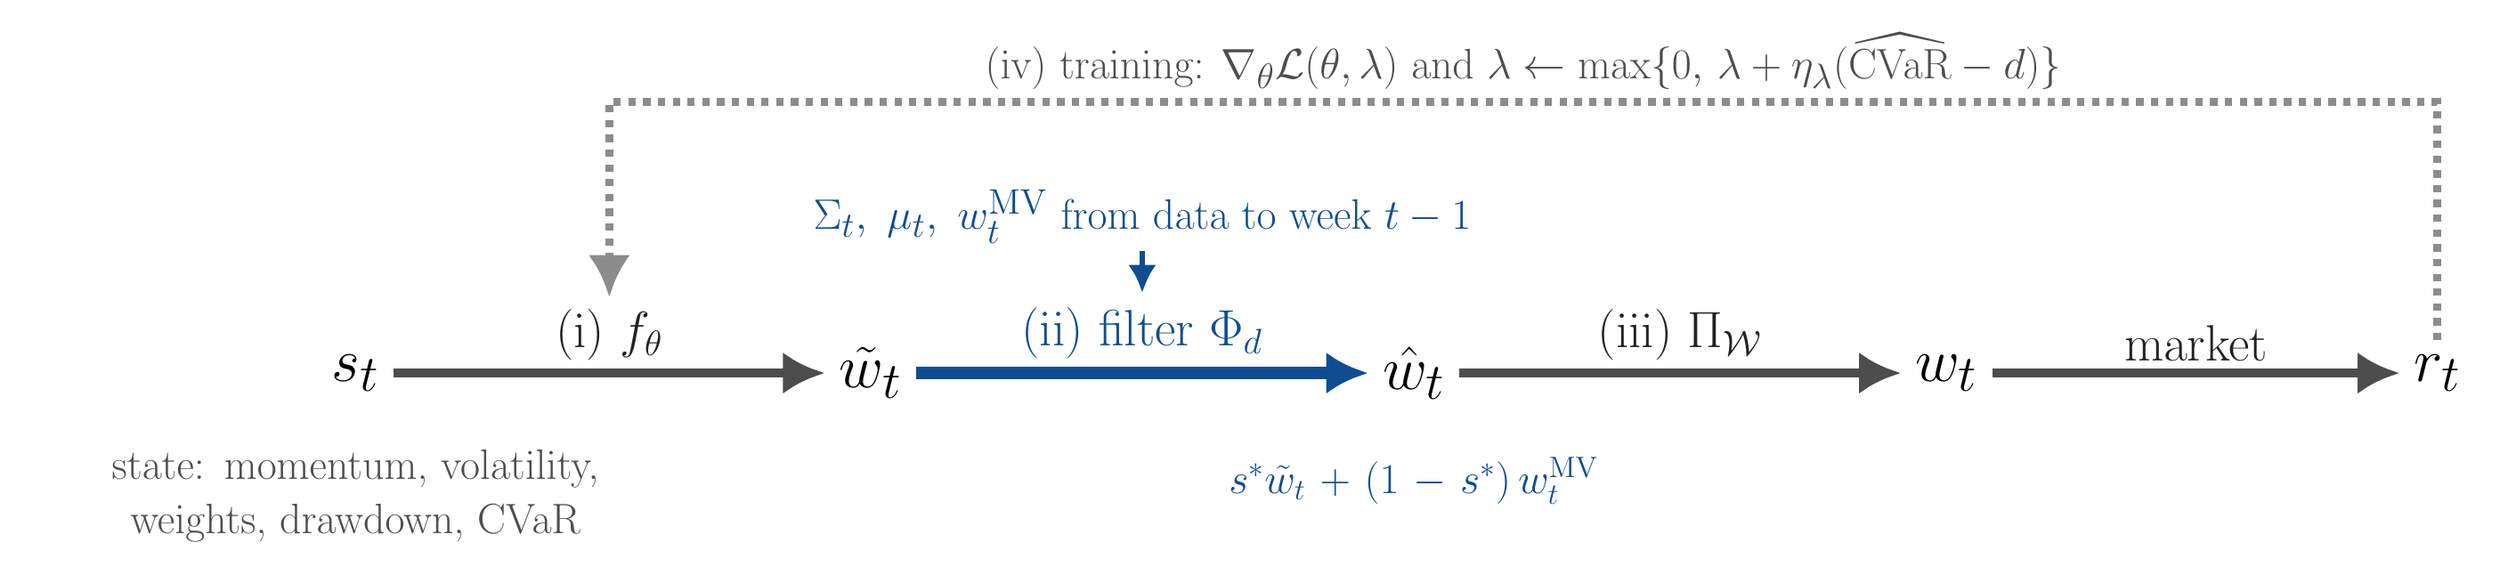
\begin{tikzpicture}[
      v/.style={font=\fontsize{30}{34}\selectfont, inner sep=2mm},
      def/.style={font=\fontsize{18.5}{22}\selectfont, text=dark, align=center, text width=74mm},
      map/.style={-{Latex[length=6mm, width=6mm]}, line width=1.2mm, color=dark},
      lab/.style={above, font=\fontsize{21}{24}\selectfont, text=ink},
      node distance=0mm]
    \node[v] (s) at (0,0) {$s_t$};
    \node[v] (wt) at (7.35,0) {$\tilde w_t$};
    \node[v] (wh) at (15.1,0) {$\hat w_t$};
    \node[v] (w) at (22.7,0) {$w_t$};
    \node[v] (r) at (29.7,0) {$r_t$};
    \draw[map] (s) -- node[lab] (fl) {(i) $f_\theta$} (wt);
    \draw[map, color=navy, line width=1.8mm] (wt) -- node[lab, text=navy] (phil) {(ii) filter $\Phi_d$} (wh);
    \draw[map] (wh) -- node[lab] {(iii) $\Pi_{\mathcal W}$} (w);
    \draw[map] (w) -- node[lab] {market} (r);
    \node[def, below=5mm of s, text width=92mm] {state: momentum, volatility,\\ weights, drawdown, CVaR};
    \node[def, below=5mm of wh, text=navy] {$s^\ast\tilde w_t+(1-s^\ast)\,w^{\mathrm{MV}}_t$};
    %% The filter's trailing inputs: data up to week t-1 only.
    \node[above=6mm of phil, font=\fontsize{19}{22}\selectfont, text=navy, inner sep=1mm] (inp)
      {$\Sigma_t,\ \mu_t,\ w^{\mathrm{MV}}_t$ from data to week $t-1$};
    \draw[-{Latex[length=4mm, width=4mm]}, line width=0.8mm, color=navy] (inp.south) -- (phil.north);
    %% Training updates the policy parameters and the multiplier.
    \draw[map, dashed, color=mid] (r.north) -- ++(0,34mm) -| node[pos=0.25, above,
      font=\fontsize{19}{22}\selectfont, text=dark]
      {(iv) training: $\nabla_\theta\mathcal{L}(\theta,\lambda)$ and
        $\lambda\leftarrow\max\{0,\,\lambda+\eta_\lambda(\widehat{\mathrm{CVaR}}-d)\}$}
      (fl.north);
  \end{tikzpicture}
  \par\figcap{Figure 5. The decision at week $t$ as a composition of maps.}
  \RaggedRight
  \begin{enumerate}[label=(\roman*), leftmargin=1.6em, itemsep=2mm]
    \item \emph{Policy.} An MLP $f_\theta$ tilts an adaptive inverse-volatility anchor $a_t$,
      $\tilde w_t=\mathrm{softmax}(\log a_t+f_\theta(s_t))$. At initialisation
      $f_\theta\approx0$, so training starts from the anchor and learns a state-dependent
      tilt.
    \item \emph{Filter.} From the trailing 104 weekly returns it forecasts
      $\widehat{\mathrm{CVaR}}(w)=c_\alpha\sigma_p(w)-\mu_p(w)$, with
      $c_\alpha=\varphi(\Phi^{-1}(\alpha))/(1-\alpha)$ and $c_{0.95}=2.06$. An over-budget
      proposal is mixed with the trailing minimum-variance portfolio $w^{\mathrm{MV}}_t$,
      keeping as much of the proposal as the budget allows,
      $s^\ast=\max\{s\in[0,1]:\widehat{\mathrm{CVaR}}(s\tilde w_t+(1-s)w^{\mathrm{MV}}_t)\le
      d\}$. It is a safety layer in the sense of [3] and uses data up to week $t-1$ only.
    \item \emph{Projection.} $\Pi_{\mathcal W}$ enforces long-only weights, $w_i\le0.40$ and
      $\lVert w_t-w_{t-1}\rVert_1\le0.50$. The market then pays $r_t$ net of a 5\,bps cost
      per unit of turnover.
    \item \emph{Training.} On random windows of past weeks we back-propagate
      \[
        \mathcal{L}(\theta,\lambda)=-\mathrm{Sharpe}(r)+\lambda\,\mathrm{ReLU}
          \big(\widehat{\mathrm{CVaR}}-d\big)+\kappa\,\mathrm{turnover},\qquad
        \lambda\leftarrow\max\{0,\ \lambda+\eta_\lambda(\widehat{\mathrm{CVaR}}-d)\},
      \]
      where $\widehat{\mathrm{CVaR}}$ is the mean of the worst 5\% of window returns, so its
      gradient reaches only tail weeks. We keep the checkpoint with the best validation
      objective among those within the validation CVaR limit.
  \end{enumerate}
  \runin{Setup} The stress test trains on 2008 to 2018 and tests on the 267 weeks from late 2019
  to 2024, with seeds 7, 13, 23, 42 and 2025. Six classical rules (equal weight, inverse
  volatility, minimum variance, mean-variance, risk parity and a min-CVaR LP) are refit weekly on
  the trailing 104 weeks.
}

\block{Results}{\body
  \runin{Decision-time filter} A larger dual step made $\lambda$ move, but the portfolio was then
  over budget in 75.1\% of test weeks. Classical rules met the same budget in 92\% of weeks, so
  the budget was attainable. Adding the filter lowered the breach rate to \hl{7.4\%} (Fig.~6).
  Raising $\lambda$ during testing without the filter left the breach rate at 81.9\%, which
  attributes the improvement to the filter.
  \fig[\linewidth]{figure_coupling.pdf}
  \figcap{Figure 6. Stress window, five-seed means. Breach is the share of test weeks over budget.}
  \runin{Tail risk across test settings} The walk-forward test retrains every 26 weeks on the
  previous six years and tests on the next 26 unseen weeks, giving 20 folds per universe from
  2015 to 2024. In Figure 7 each fold is one point. Below the diagonal the constraint lowered
  $\mathrm{CVaR}_{0.99}$. On it the budget never bound, so both models held the same portfolio.
  \par\smallskip\noindent
  \begin{minipage}[b]{0.4\linewidth}\centering
    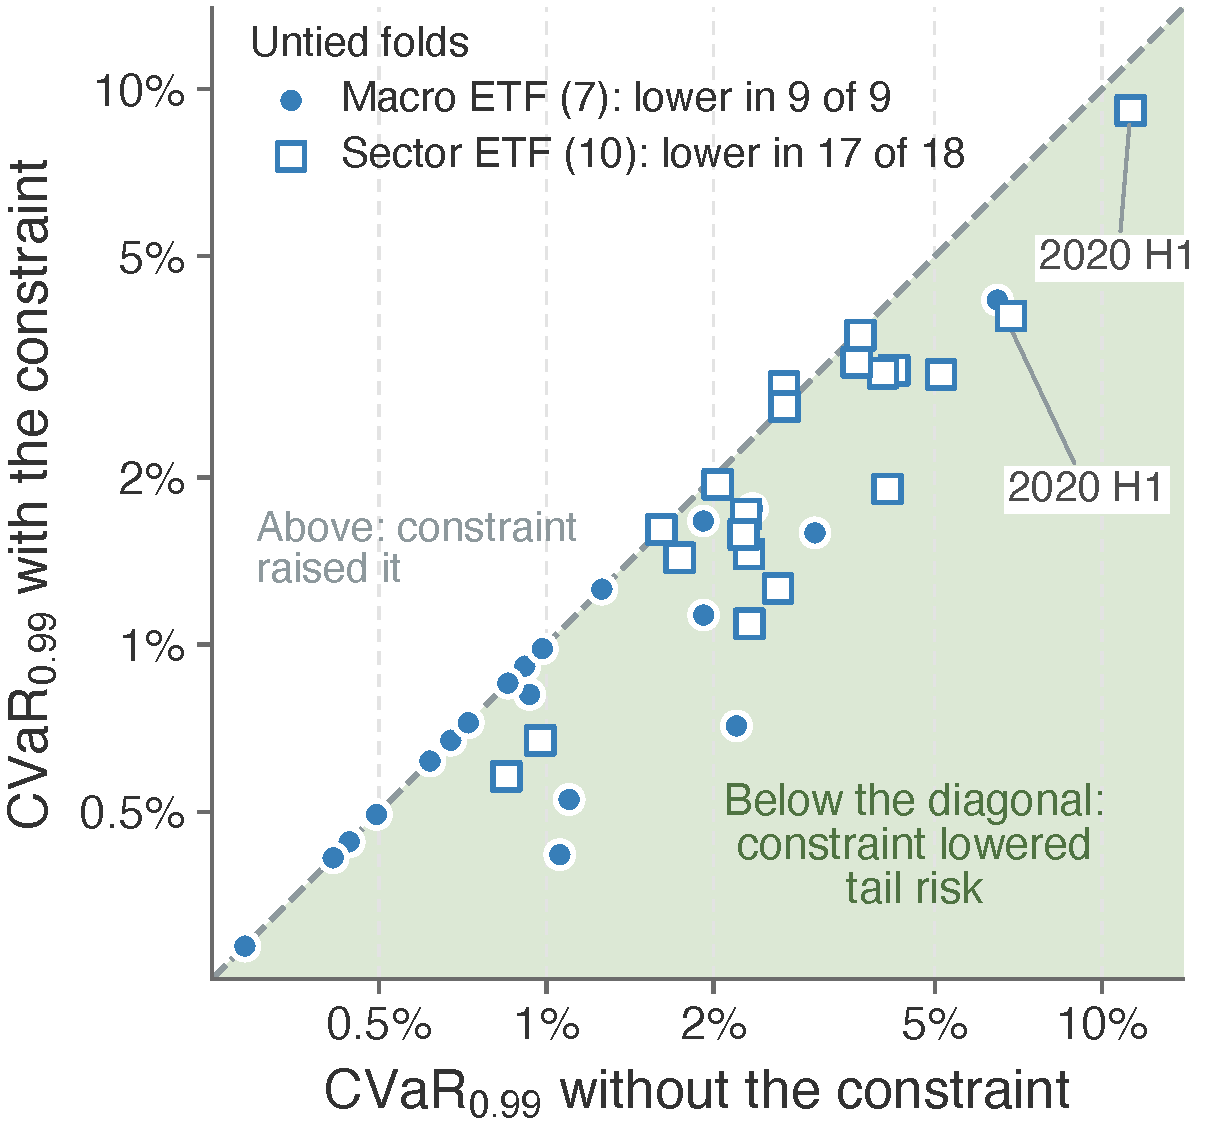
\includegraphics[width=\linewidth]{figure_fold_scatter.pdf}
    \figcap{Figure 7. Walk-forward folds, $\mathrm{CVaR}_{0.99}$ without against with the
    constraint (log scale).}
  \end{minipage}\hfill
  \begin{minipage}[b]{0.56\linewidth}\centering
    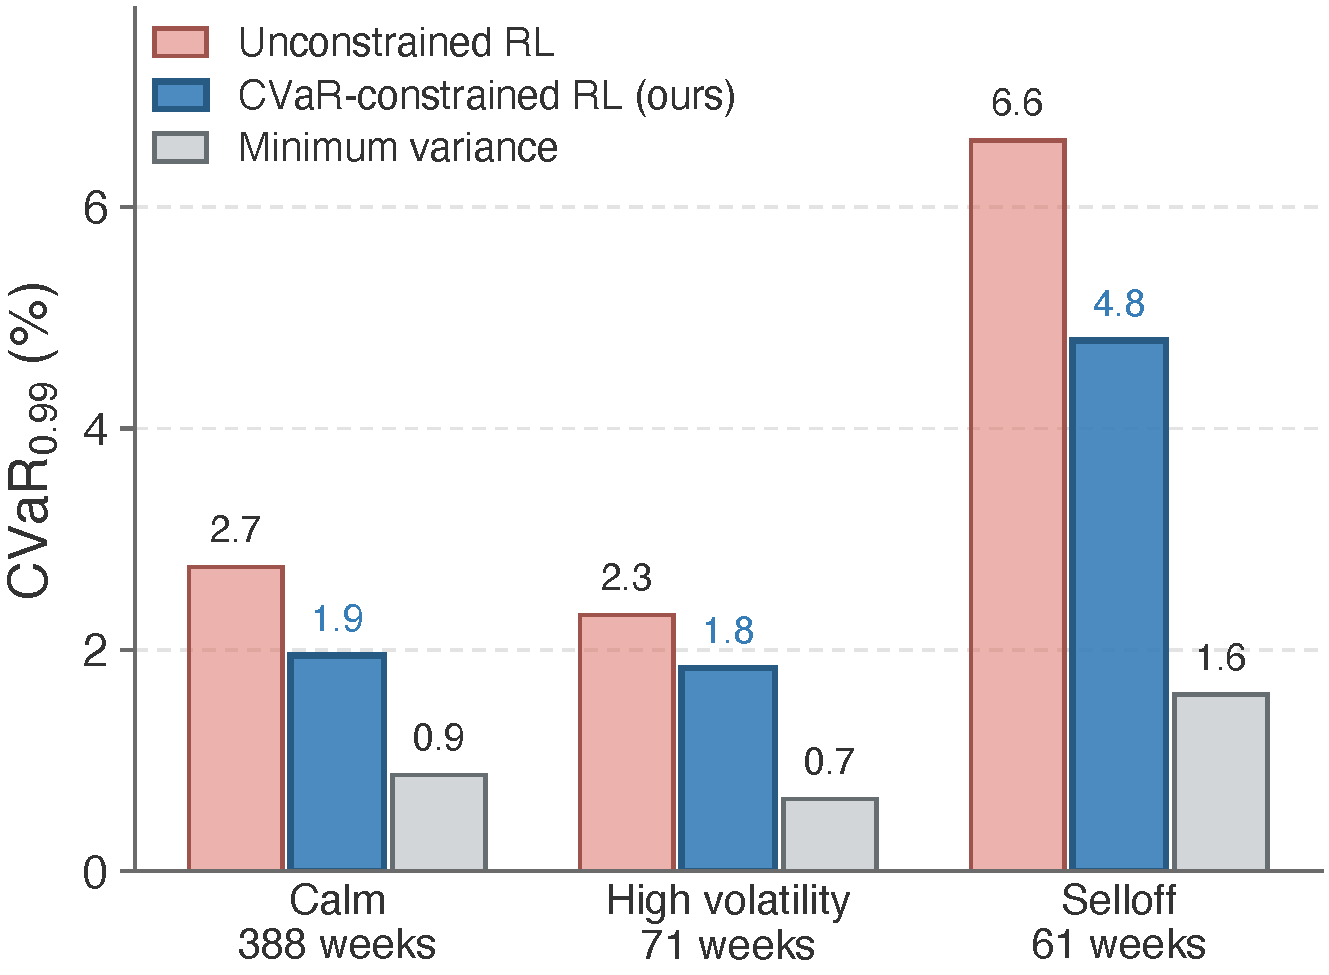
\includegraphics[width=\linewidth]{figure_regime.pdf}
    \figcap{Figure 8. Out-of-sample $\mathrm{CVaR}_{0.99}$ by market regime, 10-fold
    walk-forward from 2010 to 2024, 7 ETFs. The constraint lowered it by 21 to 29\% in every
    regime.}
  \end{minipage}\par
  \bigskip
  \tabcap{Table 1. $\mathrm{CVaR}_{0.99}$ (\%) without (unc.) and with (con.) the constraint.}
  \smallskip
  {\fontsize{21}{26}\selectfont\setlength{\tabcolsep}{4.5mm}\renewcommand{\arraystretch}{1.4}\noindent
  \begin{minipage}[t]{0.47\linewidth}\centering
    \textit{Stress window, 267 test weeks}\par\medskip
    \begin{tabular}{@{}lcrrc@{}}
      \toprule
      Universe & seeds & unc. & con. & 95\% CI (pp) \\
      \midrule
      7 ETFs & 5 & 6.47 & 3.27 & $[-3.5,\,-2.2]$ \\
      10 sector ETFs & 3 & 10.9 & 7.6 & $[-5.0,\,-3.2]$ \\
      \bottomrule
    \end{tabular}
  \end{minipage}\hfill
  \begin{minipage}[t]{0.49\linewidth}\centering
    \textit{Walk-forward, 20 folds per universe}\par\medskip
    \begin{tabular}{@{}lrrrr@{}}
      \toprule
      Universe & unc. & con. & lower & $p$ \\
      \midrule
      7 ETFs & 1.43 & 1.02 & 9/9 & 0.0077 \\
      10 sector ETFs & 3.36 & 2.50 & 17/18 & 0.0003 \\
      \hl{Both, pooled} & \hl{2.40} & \hl{1.76} & \hl{26/27} & \hl{$8.8\times10^{-6}$} \\
      \bottomrule
    \end{tabular}
  \end{minipage}\par}
  \medskip
  {\centering\fontsize{17}{21}\selectfont\color{dark}
  CI: 95\% bootstrap, seed 7. Lower: folds improved, ties excluded. $p$: Wilcoxon signed-rank.\par}
}

\block{Limitations and future work}{\body
  \runin{Limitations} The evidence is limited to two equity-centric ETF universes at weekly
  frequency, under proportional transaction costs without market impact or borrowing costs. The
  filter relies on a Gaussian approximation to forward CVaR, which may understate losses when
  returns are fat-tailed, and it achieves compliance partly by holding portfolios close to
  minimum variance (mean $L_1$ distance 0.48 to 0.61). The constrained learner underperformed
  minimum variance in selloff weeks (Sharpe $-0.809$ against 0.035), its out-of-sample Sharpe
  advantage over classical baselines did not survive deflation, and the protocol reversal is
  documented on a single 31-asset window.

  \runin{Future work} Replacing the Gaussian forecast with a semi-parametric or extreme-value
  estimate of tail risk would test whether breach depth can be reduced further. An adaptive dual
  update, such as the PID Lagrangian of [7], could remove the need to tune $\eta_\lambda$
  against the scale of the CVaR excess. Evaluation on daily data with market-impact costs, on
  non-equity universes and over multiple rolling start dates would establish how generally the
  breach reduction and the protocol reversal hold.
  \par\medskip
  {\RaggedRight\fontsize{16}{19.5}\selectfont\color{dark}
    \textbf{References.}
    [1] R.\,T. Rockafellar, S. Uryasev. Optimization of conditional value-at-risk.
    \emph{J.\ Risk} 2 (2000).
    [2] E. Altman. \emph{Constrained Markov Decision Processes}. 1999.
    [3] G. Dalal et al. Safe exploration in continuous action spaces. arXiv:1801.08757, 2018.
    [4] D.\,H. Bailey, M. L\'opez de Prado. The deflated Sharpe ratio. \emph{JPM} 40 (2014).
    [5] O. Ledoit, M. Wolf. A well-conditioned estimator for large-dimensional covariance
    matrices. \emph{JMVA} 88 (2004).
    [6] Y. Benjamini, Y. Hochberg. Controlling the false discovery rate. \emph{JRSS B} 57
    (1995).
    [7] A. Stooke, J. Achiam, P. Abbeel. Responsive safety in RL by PID Lagrangian methods.
    ICML 2020.\par\smallskip
    \envelope\ nl2992@columbia.edu\quad
    yh3915@columbia.edu\par}
}
\end{columns}

\end{document}
